\documentclass[12pt]{article}

% --- Paquetes Requeridos para Estilo APA y Formato ---
\usepackage[spanish,es-tabla]{babel} % Configuración para idioma español y etiquetas de tablas
\usepackage{geometry}
\geometry{
    a4paper,
    margin=1in % Margen de 1 pulgada (2.54 cm) requerido por APA
}

\usepackage{setspace}
\doublespacing % Espaciado doble requerido por APA
\usepackage{fontspec} % Requerido en LuaLaTeX para fuentes tipográficas
\setmainfont{Times New Roman} % Configura Times New Roman de forma nativa para LuaLaTeX (corrige negritas)
\usepackage{indentfirst} % Indentación en el primer párrafo de cada sección
\usepackage{titlesec}
\usepackage{graphicx}
\usepackage{booktabs} % Para tablas limpias estilo APA (sin líneas verticales)
\usepackage{caption}
\usepackage{float} % Para posicionamiento preciso de tablas e imágenes (H)
\usepackage{hyperref}
\usepackage{xurl}
\usepackage{fancyhdr}

% --- Configuración de Encabezado y Pie de Página (APA 7 Estudiantes) ---
\pagestyle{fancy}
\fancyhf{}
\setlength{\headheight}{15pt} % Aumenta la altura del encabezado para evitar advertencias de fancyhdr
\addtolength{\topmargin}{-3pt} % Compensa el cambio de altura del encabezado
\rhead{\thepage} % Número de página en la esquina superior derecha
\lhead{}
\renewcommand{\headrulewidth}{0pt} % Elimina la línea horizontal del encabezado

% --- Configuración de Títulos estilo APA 7 (Evita duplicidad de numeración) ---
\titleformat{\section}{\normalfont\normalsize\bfseries\centering}{}{0pt}{}
\titleformat{\subsection}{\normalfont\normalsize\bfseries}{}{0pt}{}
\titleformat{\subsubsection}{\normalfont\normalsize\bfseries\itshape}{}{0pt}{}

% Ajustes de sangría de párrafos (0.5 pulgadas)
\setlength{\parindent}{0.5in}
\setlength{\parskip}{0pt}

% --- Formato APA para Leyendas de Tablas y Figuras ---
\captionsetup[table]{
    labelfont=bf,
    textfont=it,
    labelsep=newline,
    justification=justified,
    singlelinecheck=false,
    skip=10pt
}
\captionsetup[figure]{
    labelfont=bf,
    textfont=it,
    labelsep=newline,
    justification=justified,
    singlelinecheck=false,
    skip=10pt
}

\begin{document}

% ==========================================
% I. CARÁTULA
% ==========================================
\begin{titlepage}
    \centering
    \setstretch{1.1}
    
    {\fontsize{14pt}{16pt}\selectfont\bfseries UNIVERSIDAD NACIONAL AGRARIA DE LA SELVA} \\
    \vspace{0.3cm}
    {\fontsize{12pt}{14pt}\selectfont\bfseries FACULTAD DE INGENIERÍA EN INFORMÁTICA Y SISTEMAS} \\
    \vspace{0.3cm}
    {\fontsize{12pt}{14pt}\selectfont\bfseries ESCUELA PROFESIONAL DE INGENIERÍA EN INFORMÁTICA Y SISTEMAS} \\
    
    \vspace{1.0cm}
    % Logos institucionales
    \begin{minipage}{0.8\textwidth}
        \centering
        
\includegraphics[width=3.5cm]{unas.png}  
        \hspace{0.8cm}  
        
\includegraphics[width=3.5cm]{fiis_unas.jpg}
        \vspace{0.5cm}
    \end{minipage}
    
    \vspace{1.0cm}
    {\fontsize{14pt}{16pt}\selectfont\bfseries INFORME DE PRODUCTO MÍNIMO VIABLE (MVP)} \\
    \vspace{0.6cm}
    {\fontsize{12pt}{14pt}\selectfont\bfseries ``SISTEMA DE GESTIÓN FINANCIERA CON INTELIGENCIA ARTIFICIAL - FINANCIA!''} \\
    
    \vspace{1.5cm}
    \begin{flushleft}
        \fontsize{12pt}{14pt}\selectfont
        \textbf{Presentado por:} \\
        \vspace{0.2cm}
        \hspace{0.5cm} Fabrizzio Fabiano Esquivel Mori \\
        \hspace{0.5cm} Diogo Aarón Alipázaga Bazán \\
        \hspace{0.5cm} Sergio Wilson Miranda Murrieta \\
        \hspace{0.5cm} Andrew Roy Ildefonso Sotelo \\
        \vspace{0.4cm}
        \textbf{Curso:} Innovación e Emprendimiento \\
        \vspace{0.4cm}
        \textbf{Docente:} Michael Mariño Gamboa \\
        \vspace{0.4cm}
        \textbf{Fecha:} 09 de julio de 2025
    \end{flushleft}
    
    \vfill
    {\fontsize{12pt}{14pt}\selectfont TINGO MARÍA – PERÚ \\ 2025}
    
\end{titlepage}

\newpage

% ==========================================
% II. DESCRIPCIÓN DEL PROBLEMA
% ==========================================
\section{II. DESCRIPCIÓN DEL PROBLEMA}

\subsection{¿Cuál es el problema?}
La gestión de finanzas personales es una tarea crítica para la estabilidad económica individual; sin embargo, la mayoría de las personas carecen de la disciplina y las herramientas adecuadas para llevar un control riguroso de sus ingresos y egresos. Las aplicaciones financieras tradicionales presentan una alta fricción debido a que exigen que el usuario registre de forma manual cada transacción (monto, categoría, establecimiento, fecha, cuenta de origen, etc.). Este proceso repetitivo y tedioso genera frustración y, en consecuencia, un rápido abandono de la herramienta. Adicionalmente, la falta de retroalimentación inteligente y personalizada hace que los usuarios no comprendan sus patrones de consumo ni sepan cómo alcanzar sus metas de ahorro de manera eficiente.

\subsection{¿Quiénes son los afectados?}
Los principales afectados son los jóvenes profesionales, trabajadores independientes (\textit{freelancers}), estudiantes universitarios y adultos jóvenes que están comenzando su vida financiera activa. Este segmento, habituado a la inmediatez y a la automatización de los servicios digitales (nativos digitales), experimenta una disonancia cognitiva cuando se ve obligado a utilizar interfaces complejas y procesos manuales para registrar sus gastos diarios.

\subsection{Evidencias obtenidas durante la validación}
Para validar la existencia y magnitud del problema, se aplicó una encuesta diagnóstica a un grupo muestra de 14 usuarios representativos. La muestra presentó una edad promedio de 26.3 años (rango entre 20 y 46 años, con un 85.7\% de los participantes concentrado entre los 20 y 29 años) y una distribución por sexo de 71.4\% hombres y 28.6\% mujeres. Los resultados revelaron las siguientes evidencias críticas:
\begin{itemize}
    \item \textbf{Uso y control actual:} El 64.3\% utiliza alguna aplicación móvil o banca digital para el seguimiento financiero, mientras que el 35.7\% no lleva ningún control global sobre sus movimientos.
    \item \textbf{Frustraciones críticas:} Entre los usuarios que utilizan plataformas tradicionales, el 44.4\% reportó serias frustraciones relacionadas con la lentitud e ineficiencia del inicio de sesión y registro (``no es rápido y toma tiempo usarlo'', ``a veces demora más de lo usual'') o con caídas recurrentes del sistema.
    \item \textbf{Falta de centralización bancaria:} Un 22.2\% destacó como principal frustración que las aplicaciones de banca móvil son cerradas y no registran de forma integrada los movimientos de otras entidades bancarias, obligándolos a realizar registros manuales separados.
    \item \textbf{Demanda de automatización con IA:} Ante la propuesta del uso de inteligencia artificial controlada por comandos de voz o texto, se obtuvo una aceptación promedio de 6.29/10. Asimismo, la posibilidad de automatizar registros mediante la lectura de actividad del celular (chats y notificaciones) recibió una puntuación de 6.21/10, evidenciando el interés en reducir el esfuerzo humano de digitación.
\end{itemize}

\newpage

% ==========================================
% III. DESCRIPCIÓN DEL MVP
% ==========================================
\section{III. DESCRIPCIÓN DEL MVP}

\subsection{Nombre del MVP}
FinancIA! — Sistema de Gestión Financiera con Inteligencia Artificial.

\subsection{Objetivo}
Facilitar el registro, control y planificación de las finanzas personales mediante un asistente virtual impulsado por inteligencia artificial y una interfaz de usuario limpia e interactiva, reduciendo al mínimo la fricción del ingreso de datos y proporcionando alertas proactivas para promover la salud financiera.

\subsection{Funcionalidades mínimas implementadas}
\begin{enumerate}
    \item \textbf{Asistente de IA (Chat):} Un módulo interactivo de chat donde el usuario escribe un mensaje simple (ej. \textit{``Gasté \$25 en Uber Trip hoy''}). La aplicación interpreta el texto en lenguaje natural, extrae automáticamente el monto, el establecimiento y la categoría de gasto, y lo registra sin intervención manual adicional.
    \item \textbf{Historial de Movimientos:} Panel integral que muestra el balance neto, los ingresos totales y los egresos acumulados en tiempo real. Incluye un historial detallado de transacciones con un buscador por establecimiento y filtros por categoría o tipo de flujo, además de permitir el registro manual.
    \item \textbf{Límites de Presupuesto:} Control de gastos por categorías con alertas de consumo progresivo utilizando un código de colores (verde para saludable, amarillo para advertencia al llegar al 75\%, y rojo al sobrepasar el 100\%). Incluye una línea temporal semanal para comparar el ritmo de gasto frente al avance de la semana.
    \item \textbf{Metas de Ahorro:} Rastreador de metas (ej. \textit{Fondo de Emergencia}) con barra de progreso interactiva, simulador de depósitos rápidos para ingresar montos ficticios y configuraciones mediante interruptores (\textit{toggles}) para recibir informes proactivos de la IA.
\end{enumerate}

\subsection{Alcance del MVP}
El alcance de este MVP se centra en el desarrollo de la interfaz de usuario web responsiva (implementada con React, TypeScript y Tailwind CSS/CSS vanilla) con un almacenamiento de datos en el estado local de la aplicación (\textit{local storage} / \textit{store}). Muestra de forma funcional los flujos completos de interacción de chat, visualización de balances, cálculo dinámico de presupuestos por categoría y simulación de ahorros sin necesidad de una infraestructura de base de datos en la nube o pasarelas de pago.

\newpage

\subsection{Evidencias Gráficas del MVP}
Las capturas de pantalla de la interfaz gráfica y los módulos del MVP (Chat con Asistente de IA, Historial de Movimientos, Límites de Presupuesto y Metas de Ahorro) se han organizado detalladamente en la sección de \textbf{Anexos} al final del documento (ver Figuras 1, 2, 3 y 4 en el Anexo A).

\newpage

% ==========================================
% IV. EARLY ADOPTERS
% ==========================================
\section{IV. EARLY ADOPTERS}

De acuerdo con las especificaciones del diseño del proyecto, en la Tabla 1 se presenta la caracterización de los usuarios seleccionados como \textit{early adopters} para las pruebas de usabilidad y validación del MVP. Cada perfil ha sido seleccionado estratégicamente para evaluar la reducción de fricción en diferentes hábitos de gestión financiera.

\begin{table}[H]
\centering
\singlespacing
\caption{Perfil y Justificación de los Early Adopters del MVP}
\label{tab:early_adopters}
\begin{tabular}{p{3.5cm}p{5.7cm}p{6cm}}
\toprule
\textbf{Usuario} & \textbf{Perfil} & \textbf{Justificación} \\
\midrule
Usuario 1 \newline José L. Mariño & Estudiante de pregrado (22 años, M). Usuario de BCP y Yape. Experimenta frustración por la falta de categorización inteligente y por realizar sumas manuales de microgastos cotidianos. & Representa al segmento estudiantil nativo digital que maneja múltiples microgastos diarios. Útil para validar la categorización inteligente y la reducción de fricción al registrar datos. \\
\addlinespace
Usuario 2 \newline Jean P. Pinedo & Trabajador independiente / Freelancer (22 años, M). Combina apps bancarias con Excel manual. Frustrado por el tiempo que quita el registro manual y la lentitud de balance de cuentas. & Representa a trabajadores independientes que requieren optimizar su tiempo diario. Permite evaluar la rapidez y centralización de balances financieros inmediatos. \\
\addlinespace
Usuario 3 \newline Frank H. Bustillos & Estudiante de pregrado (23 años, M). Usuario de Yape. Frustrado por la gestión fragmentada al no poder consolidar movimientos de múltiples tarjetas de otros bancos. & Clave para validar la necesidad de centralización de balances generales y probar la usabilidad de la interfaz conversacional para consolidar gastos diversos. \\
\addlinespace
Usuario 4 \newline Augusto Arias & Estudiante de pregrado (22 años, M). No utiliza ninguna aplicación de control financiero por considerarlas sumamente lentas, tediosas y con formularios extensos y complejos. & Representa al perfil escéptico que rechaza las herramientas financieras tradicionales. Permite evaluar si el canal conversacional con IA elimina la barrera de adopción. \\
\addlinespace
Usuario 5 \newline Jennifer Esquivel & Emprendedora / Comerciante (38 años, F). Usuaria de la app de Banco de la Nación. Frustrada por la interfaz obsoleta, inicio lento y falta de gráficos para sus metas de ahorro. & Aporta la perspectiva de un perfil de mayor edad y orientación comercial que busca planificar metas específicas de ahorro y demanda una visualización interactiva y estimulante. \\
\bottomrule
\end{tabular}
\end{table}

\newpage

% ==========================================
% V. VALIDACIÓN DEL MVP
% ==========================================
\section{V. VALIDACIÓN DEL MVP}

\subsection{Metodología}
La validación del MVP se estructuró para evaluar la usabilidad, la fricción del usuario y el cumplimiento del objetivo principal del sistema mediante un cuestionario estandarizado.
\begin{itemize}
    \item \textbf{Fecha de prueba:} Las sesiones de prueba y recolección de encuestas se desarrollaron del 2 de julio al 6 de julio de 2025.
    \item \textbf{Número de usuarios:} Se evaluó a una muestra de 5 usuarios seleccionados bajo los perfiles de early adopters del sistema.
    \item \textbf{Actividades realizadas:}
    \begin{enumerate}
        \item \textit{Fase de inducción y perfilado:} Se registró la información demográfica (edad, sexo) y de hábitos financieros de cada participante para contextualizar su perfil.
        \item \textit{Test de interacción con el MVP:} Los usuarios interactuaron libremente con el chatbot conversacional para registrar gastos en lenguaje natural, y navegaron por los módulos de historial, límites presupuestarios y metas de ahorro.
        \item \textit{Aplicación de la encuesta de validación:} Al finalizar las pruebas, cada usuario completó el cuestionario estructurado en la plataforma Microsoft Forms para evaluar cuantitativamente y cualitativamente las funcionalidades.
    \end{enumerate}
\end{itemize}

\subsection{Resultados}
Los resultados cuantitativos y cualitativos obtenidos a partir del cuestionario aplicado a los 5 participantes se presentan en la Tabla 2.

\begin{table}[H]
\centering
\caption{Resultados de la Encuesta y Cuestionario de Validación del MVP}
\label{tab:resultados_validacion}
\begin{tabular}{p{5.5cm}p{9.3cm}}
\toprule
\textbf{Pregunta / Métrica Clave} & \textbf{Resultado y Análisis de Datos} \\
\midrule
¿Usa actualmente alguna aplicación de seguimiento financiero? & El 80\% (4 de 5) utiliza herramientas móviles. El 20\% no cuenta con ninguna herramienta de control. \\
\addlinespace
¿El registro por chat e IA redujo la fatiga de la digitación manual? & El 100\% indicó que la interfaz conversacional resolvió con éxito la fricción y pereza de la entrada tradicional de datos. \\
\addlinespace
Nivel de facilidad de uso del chatbot de IA y navegación general (1-5) & Se obtuvo una calificación promedio de \textbf{4.6 / 5.0} (92\% de satisfacción), destacando la claridad y la inmediatez. \\
\addlinespace
Utilidad de la visualización de presupuestos mediante semáforos & El 80\% lo calificó como muy intuitivo para el control diario. El 20\% sugirió presentarlo de otra forma. \\
\addlinespace
Nivel de utilidad del módulo de metas de ahorro (Escala 1-5) & Se obtuvo un promedio de \textbf{4.4 / 5.0}, valorando el simulador de depósitos rápidos y la configuración de reportes de IA. \\
\addlinespace
Requerimientos de seguridad indispensables elegidos por los usuarios & El 60\% prefiere autenticación biométrica (huella/Face ID) y el 40\% prefiere verificación en dos pasos (2FA/SMS). \\
\addlinespace
Probabilidad de adoptar la app como herramienta principal (0-10) & Puntuación promedio de \textbf{8.4 / 10}. El 100\% de los usuarios valoró la probabilidad con 8 o más, mostrando alta intención de uso. \\
\bottomrule
\end{tabular}
\end{table}

\subsection{Evidencias de Validación}
Como soporte de las pruebas de validación realizadas, las respuestas individuales fueron consolidadas y registradas digitalmente. El diseño del cuestionario de validación y el acceso al formulario de recolección oficial se encuentran referenciados detalladamente en el \textbf{Anexo B} de este informe. Asimismo, el detalle individualizado de las respuestas cualitativas de cada evaluador se encuentra organizado en las bitácoras de respuestas del entregable.

\newpage

% ==========================================
% VI. RETROALIMENTACIÓN Y MEJORAS
% ==========================================
\section{VI. RETROALIMENTACIÓN Y MEJORAS}

En la Tabla 3 se detallan los datos recolectados de cada uno de los cinco early adopters.

\begin{table}[H]
\centering
\singlespacing
\caption{Retroalimentación de Usuarios y Propuestas de Mejora del MVP}
\label{tab:retroalimentacion_mejoras}
\begin{tabular}{p{3.5cm}p{5.8cm}p{5.9cm}}
\toprule
\textbf{Early Adopter} & \textbf{Observación Realizada} & \textbf{Mejora Propuesta} \\
\midrule
Usuario 1 \newline José L. Mariño & Observó que las categorías de presupuesto predefinidas son fijas. Desea agrupar gastos de fotocopias o libros en una categoría específica de ``Educación''. & Permitir la creación y edición de categorías de gasto personalizadas a través de comandos de chat o en la interfaz de Límites. \\
\addlinespace
Usuario 2 \newline Jean P. Pinedo & La interfaz de chat es rápida y cómoda, pero desearía un recordatorio semanal proactivo sobre el estado del presupuesto sin tener que ingresar a la app. & Diseñar un sistema de notificaciones externas de la IA (vía Telegram o correo electrónico) con resúmenes de rendimiento. \\
\addlinespace
Usuario 3 \newline Frank H. Bustillos & Al cometer un error de escritura en el chat (ej. poner un cero de más), no pudo corregirlo directamente en la ventana de conversación. & Implementar un botón de ``Deshacer'' (\textit{Undo}) o edición rápida en la misma tarjeta generada por el chat. \\
\addlinespace
Usuario 4 \newline Augusto Arias & Registrar manualmente o por chat cada gasto del negocio resulta demandante. Considera vital la sincronización bancaria automática. & Desarrollar integraciones con APIs de banca abierta (\textit{Open Banking}) para sincronización de saldos y movimientos bancarios. \\
\addlinespace
Usuario 5 \newline Jennifer Esquivel & El simulador de ahorros incrementa el total acumulado, pero se pierde el registro cronológico de los depósitos ficticios ingresados. & Crear una pestaña de ``Historial de Depósitos'' en el módulo de Ahorros para listar montos y fechas de aportaciones a metas. \\
\bottomrule
\end{tabular}
\end{table}

\newpage

% ==========================================
% VII. CONCLUSIONES
% ==========================================
\section{VII. CONCLUSIONES}

\begin{itemize}
    \item \textbf{Conclusión 1:} La validación del MVP de FinancIA! demuestra que la adopción de interfaces conversacionales y procesamiento de lenguaje natural simplifica dramáticamente el registro de transacciones, reduciendo la fricción principal que causa el abandono de las aplicaciones de finanzas personales tradicionales.
    \item \textbf{Conclusión 2:} La incorporación de elementos visuales dinámicos de semaforización presupuestaria y barras de progreso gamificadas para el ahorro promueve el autocontrol del gasto y facilita una lectura rápida del estado financiero, logrando una excelente aceptación por parte del grupo de early adopters.
    \item \textbf{Conclusión 3:} La retroalimentación detallada provista por los usuarios constituye una guía clara de prioridades de desarrollo para futuras iteraciones de producto, destacando la necesidad de incorporar flujos de corrección ágiles, categorías configurables y la automatización mediante la conexión a cuentas bancarias del usuario.
\end{itemize}

\newpage

% ==========================================
% VIII. ANEXOS
% ==========================================
\section{VIII. ANEXOS}

\subsection{Anexo A: Evidencias Gráficas del MVP}
En esta sección se presentan las capturas de pantalla de la interfaz de usuario web interactiva desarrollada para el MVP del sistema FinancIA!:

\begin{figure}[H]
    \centering
    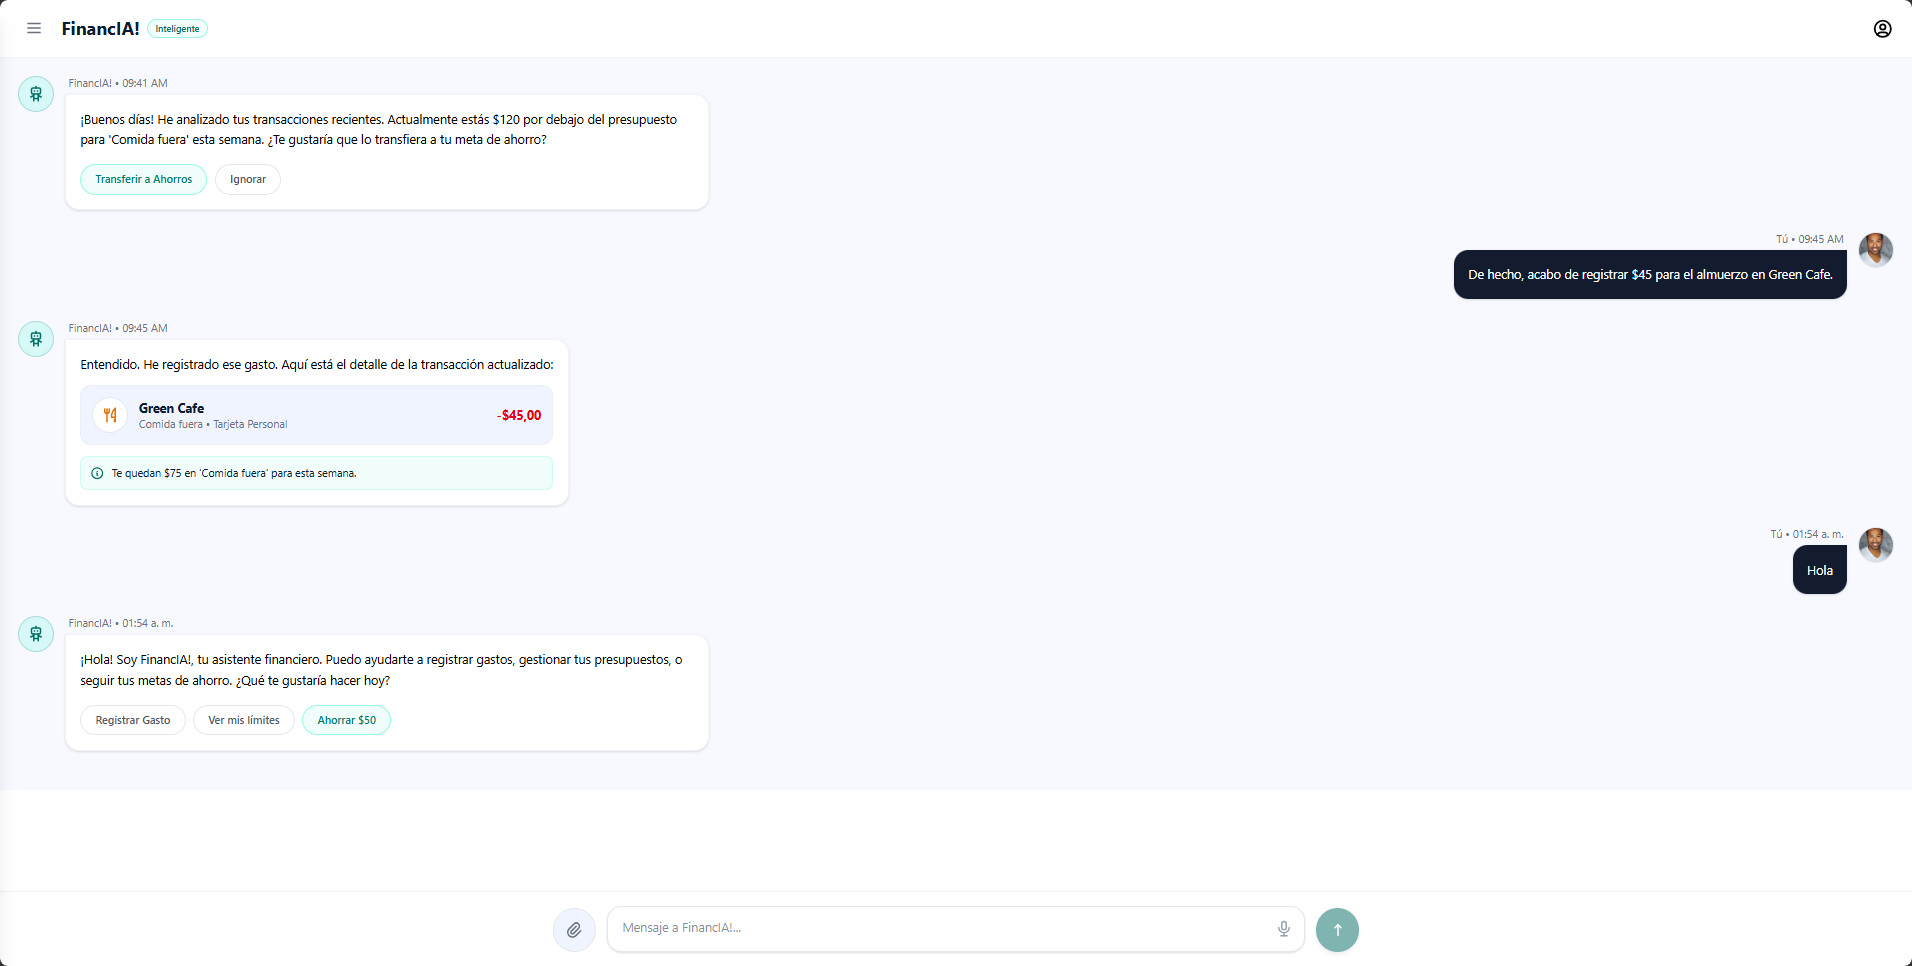
\includegraphics[width=0.85\textwidth]{chat_screenshot.png}
    \caption{Interfaz del Chat con Asistente de IA para el Registro Conversacional.}
    \label{fig:chat_ia}
\end{figure}

\begin{figure}[H]
    \centering
    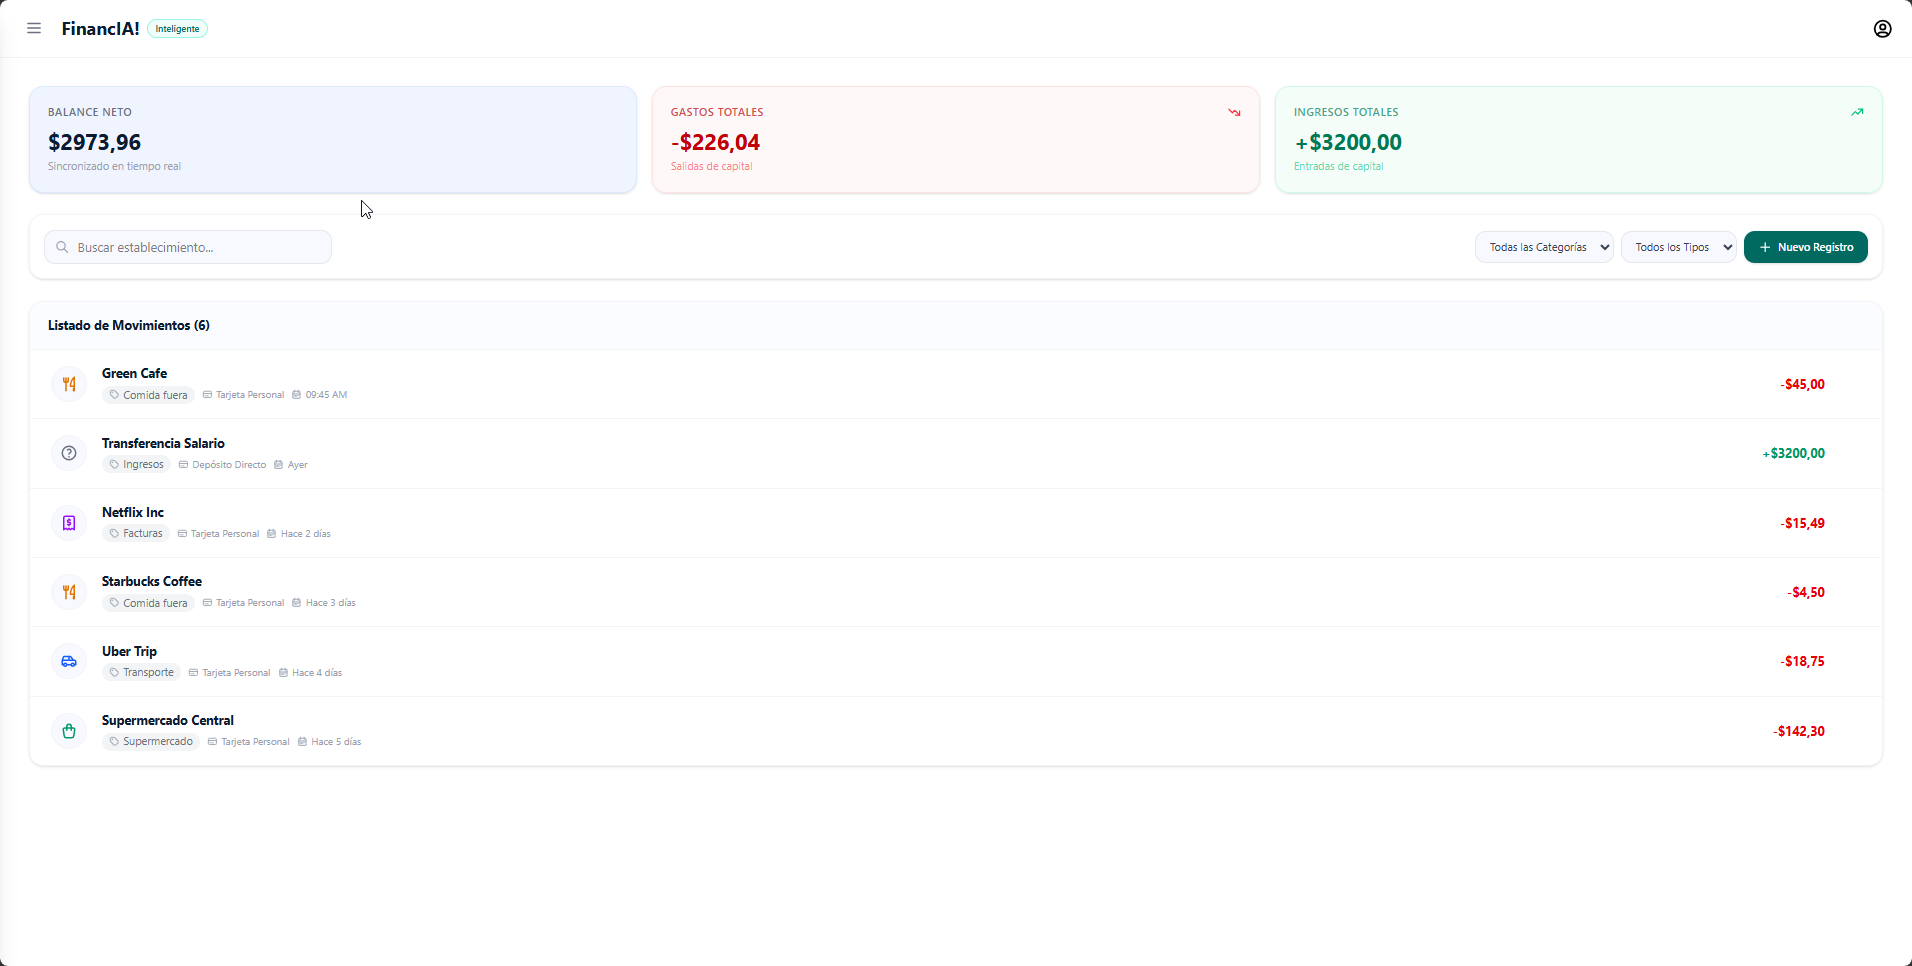
\includegraphics[width=0.85\textwidth]{movimientos_screenshot.png}
    \caption{Historial de Movimientos y Visualizador de Balances Generales.}
    \label{fig:movimientos}
\end{figure}

\begin{figure}[H]
    \centering
    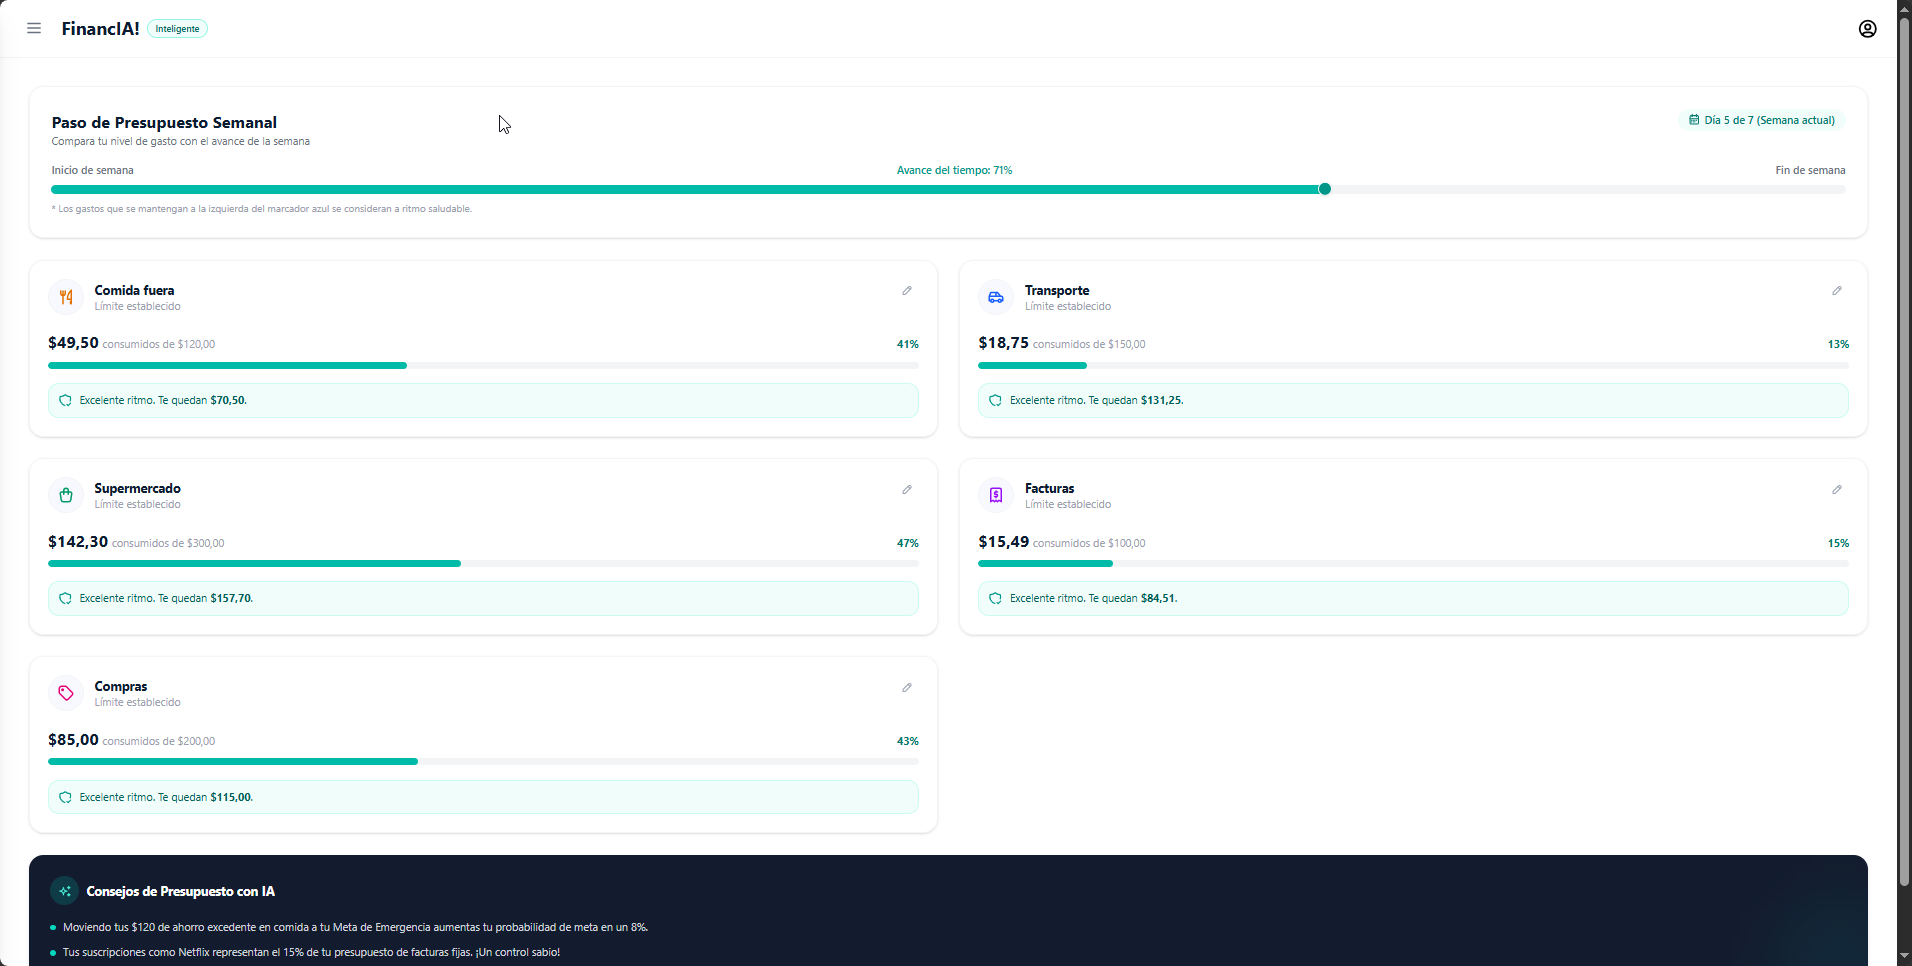
\includegraphics[width=0.85\textwidth]{limites_screenshot.png}
    \caption{Panel de Control de Presupuestos y Progreso Semanal.}
    \label{fig:limites}
\end{figure}

\begin{figure}[H]
    \centering
    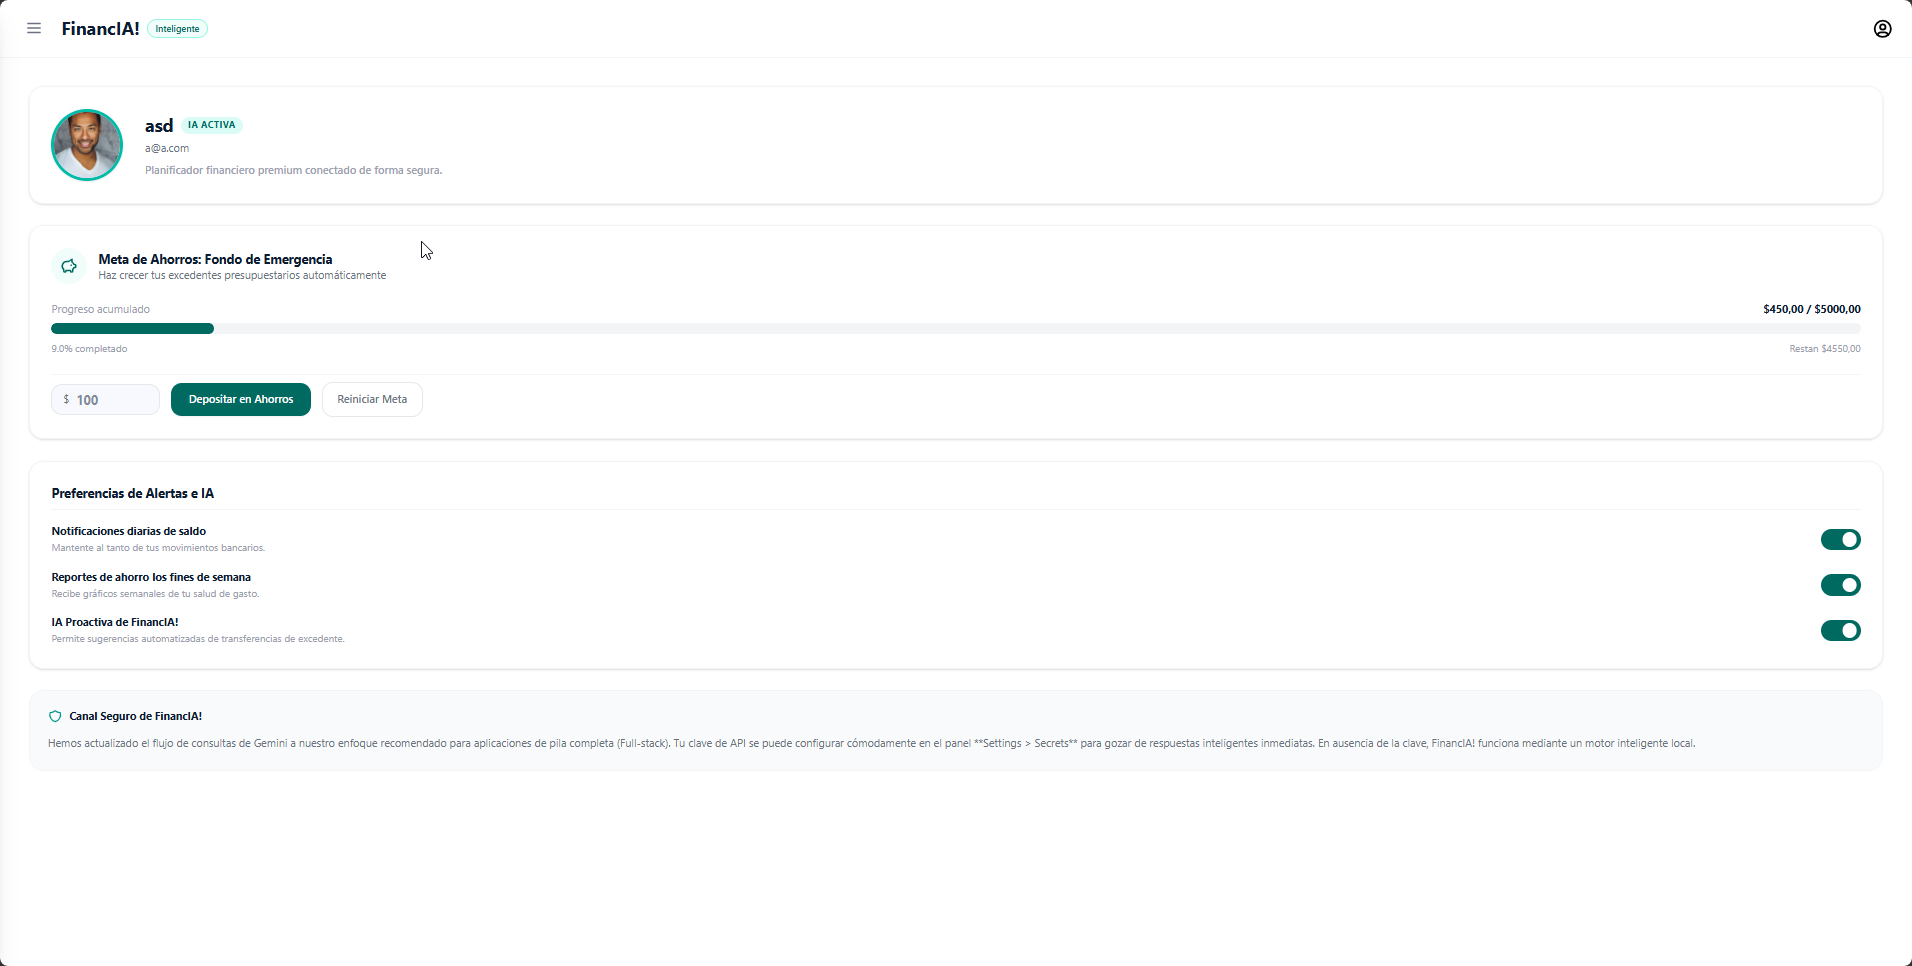
\includegraphics[width=0.85\textwidth]{ahorros_screenshot.png}
    \caption{Módulo de Metas de Ahorro y Configuración de Alertas.}
    \label{fig:ahorros}
\end{figure}

\newpage

\subsection{Anexo B: Enlaces de Acceso y Recursos del Proyecto}

\textbf{Diseño y Estructura del Formulario de Validación:} \\
El cuestionario de validación utilizado para evaluar y recopilar la retroalimentación de los \textit{early adopters} puede ser consultado en el siguiente enlace oficial de Microsoft Forms: \\
\url{https://forms.cloud.microsoft/Pages/DesignPageV2.aspx?subpage=design&FormId=hRKP4i9nlEifTkQnO7tnaoRl3E9-FVFFs-pVqsR7SJlUQTRZNUM1V00yWVM4V1hDRzkyOUhNWEVLNy4u&Token=b98f512aea074831abc82839cd40fbc1}

\vspace{0.8cm}

\textbf{Repositorio de Código Fuente del MVP (GitHub):} \\
El código fuente de la aplicación, que incluye la implementación interactiva en React, TypeScript y estilos, está alojado públicamente en el siguiente repositorio de GitHub: \\
\url{https://github.com/DiogoAlip/AI-powered-Wallet}

\end{document}
